\documentclass[tikz,border=10pt]{standalone}
\usepackage{tikz}
\usetikzlibrary{positioning}
\usepackage{tikz-feynman}
\begin{document}

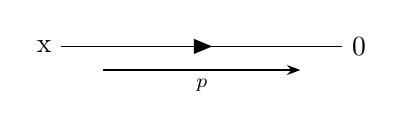
\begin{tikzpicture}[baseline]
	\begin{feynman}
		%% fig a
		\vertex (a1) at (0,0){x};
		\vertex[right =1cm  of a1] (a2);
		\vertex[right =2cm  of a1] (a3);
		\vertex[right =3cm  of a1] (a4);
		\vertex[right =4cm  of a1] (a5){0};
		% 对各个顶点连线
		\diagram*{
		{ [edge=fermion]
		(a1) --[momentum'={\scriptsize \(p\)}]  (a5),
		},
		};
	\end{feynman}
\end{tikzpicture}

\end{document}
